\chapter{Appendix}

\begin{figure}[!htb]
\centering
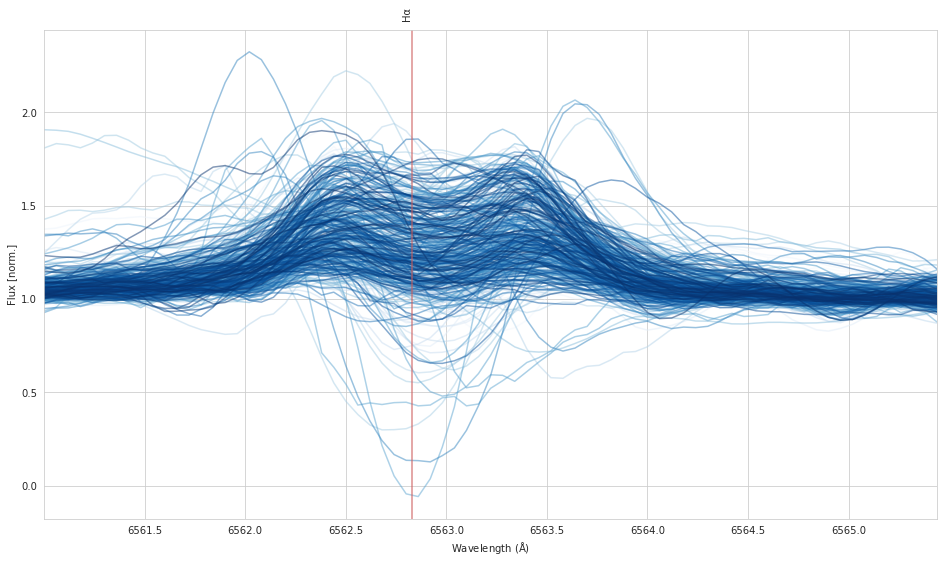
\includegraphics[scale=0.42]{figures/cotar_class_4_10.png}
\caption{A cluster of double-peaked spectra identified using DTW in the sample provided by \citet{vcotar2021galah}.}
\end{figure}

\begin{figure}[!htb]
\centering
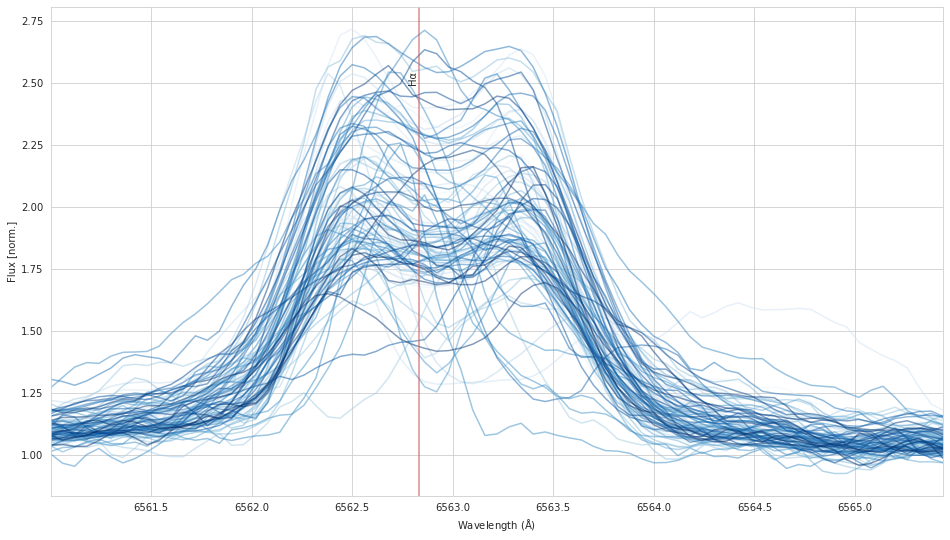
\includegraphics[scale=0.42]{figures/cotar_class_6_10.png}
\caption{A cluster of double-peaked spectra identified using DTW in the sample provided by \citet{vcotar2021galah}.}
\end{figure}

\begin{figure}[!htb]
\centering
\includegraphics[scale=0.10]{figures/t-sne halpha masked with cotar.png}
\caption{t-SNE map for all spectra in DR3 with H$\upalpha$ emission-line spectra identified by \citet{vcotar2021galah} tagged in pink.}
\end{figure}

\begin{figure}[!htb]
\centering
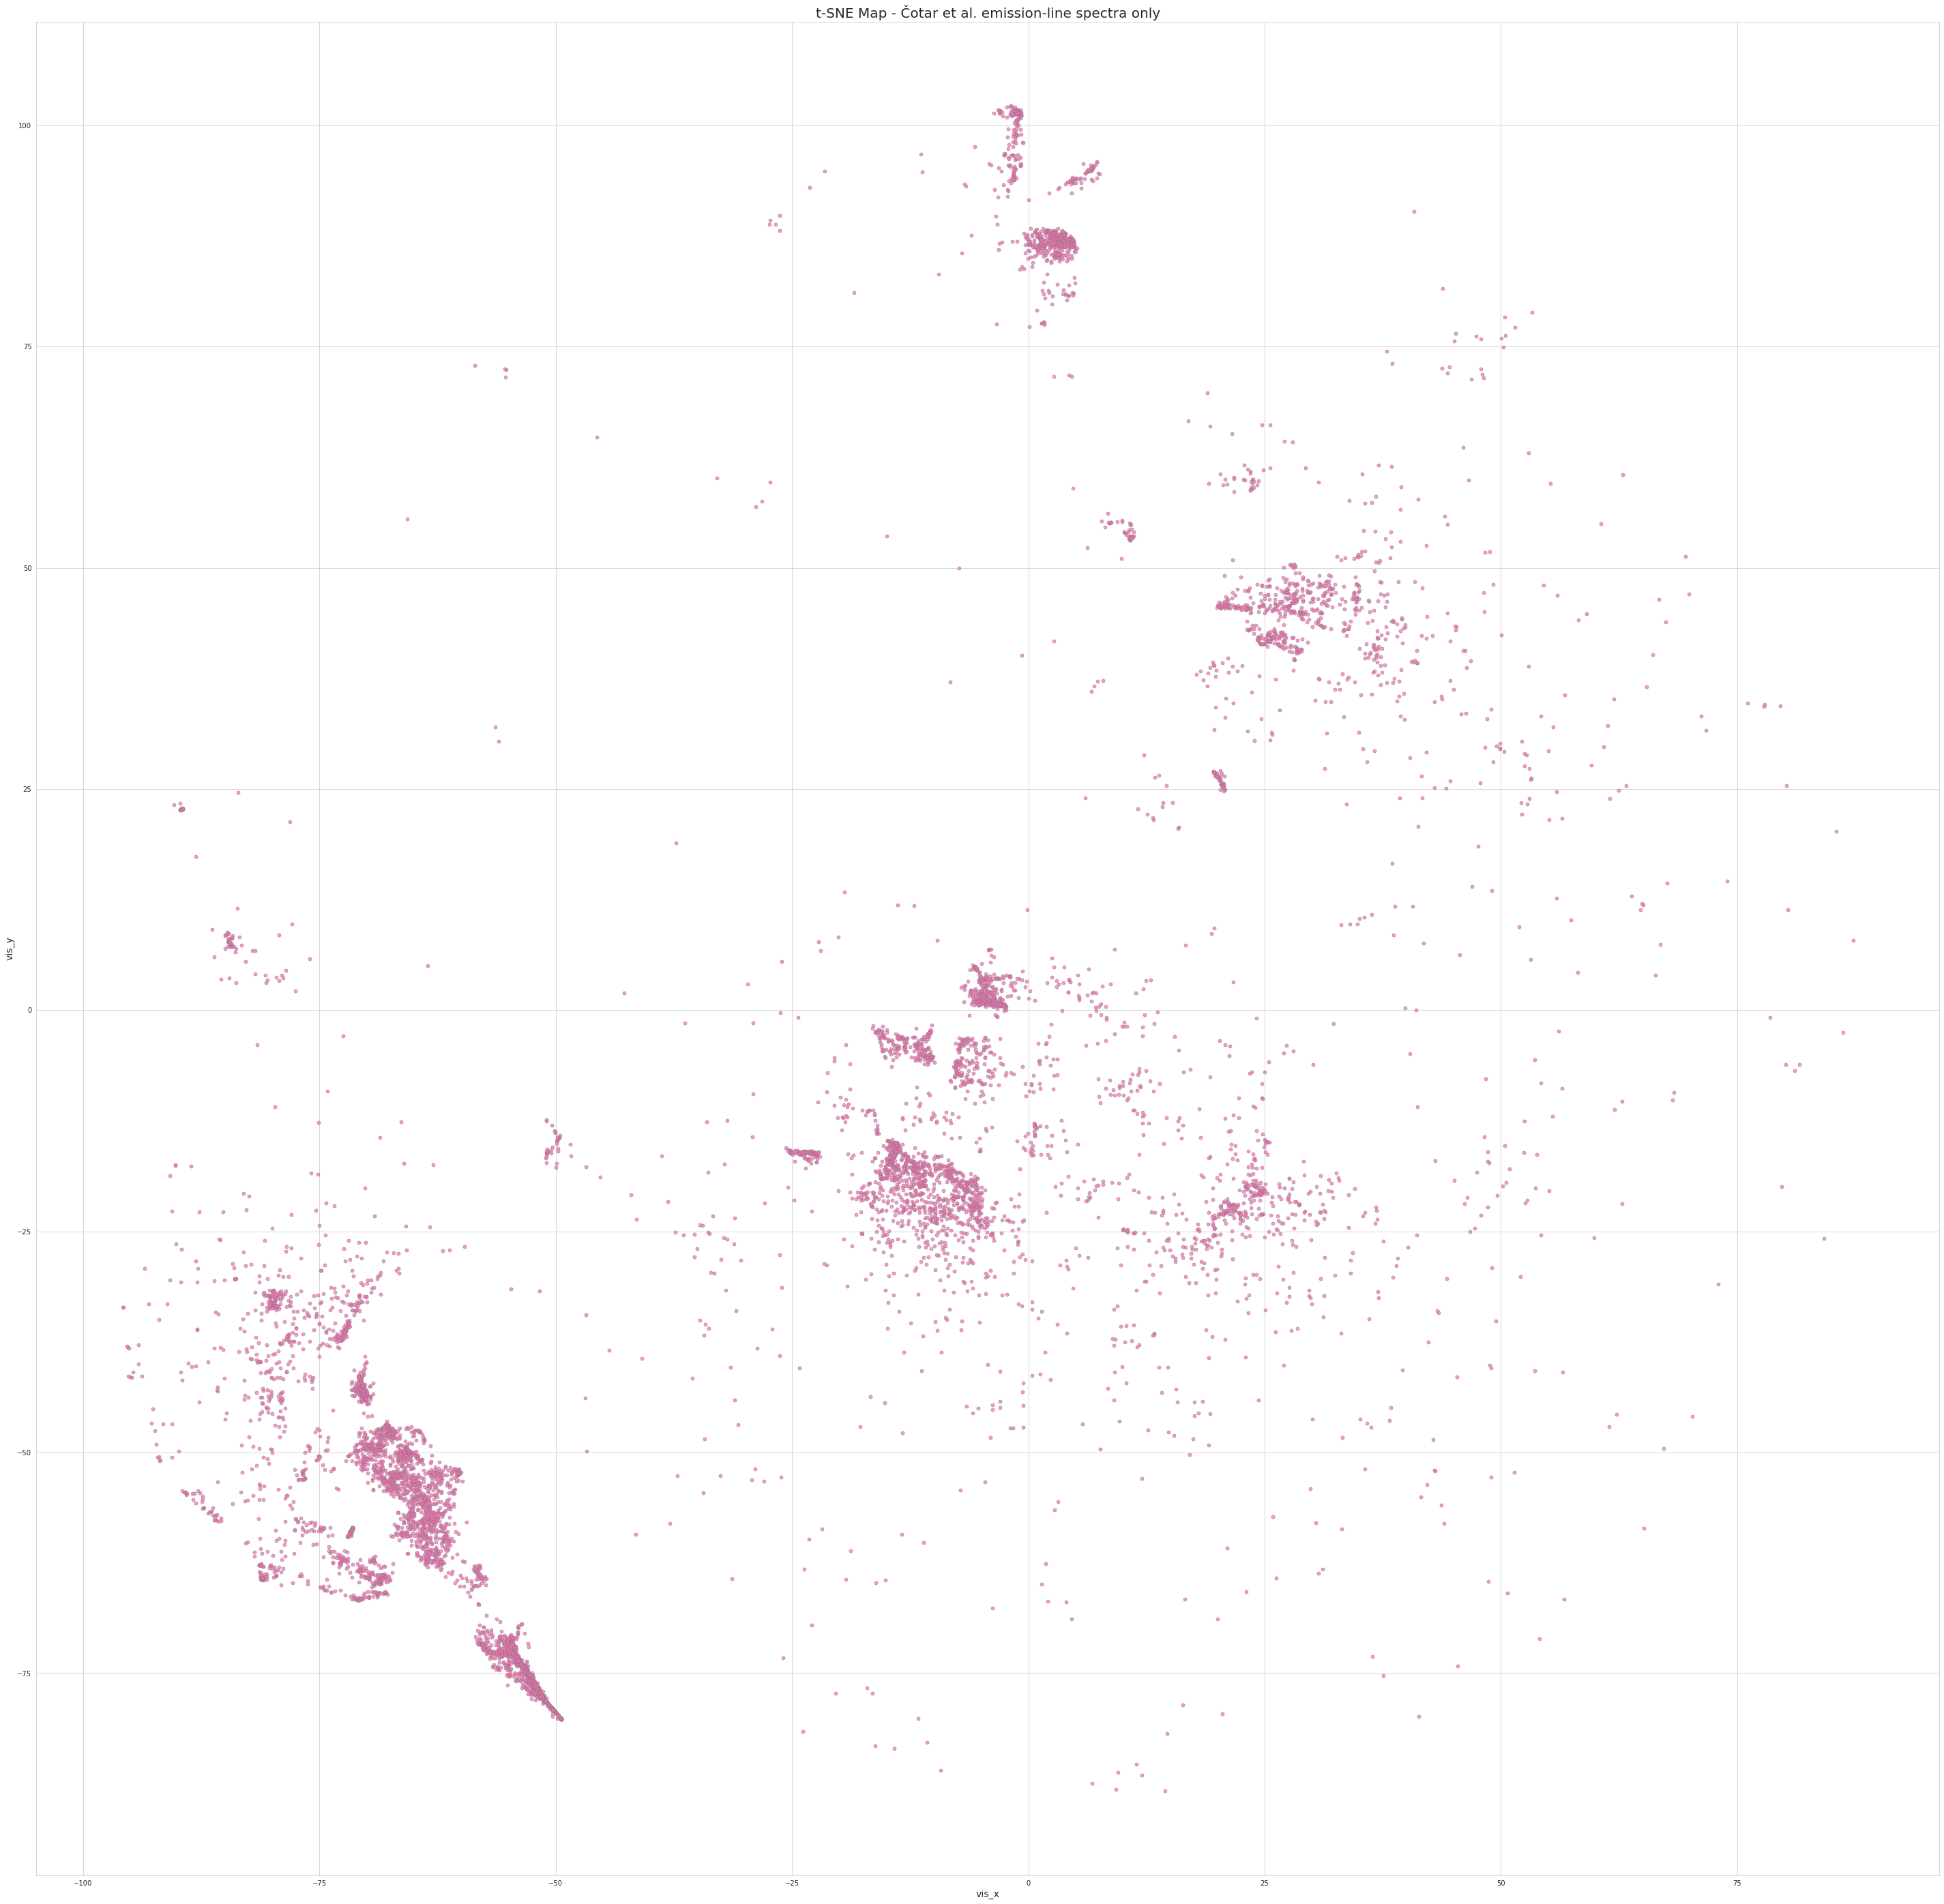
\includegraphics[scale=0.10]{figures/tsne_cotar_only.png}
\caption{H$\upalpha$ emission-line spectra identified by \citet{vcotar2021galah}, projected to the same t-SNE map, excluding presumably typical spectra.}
\end{figure}

\begin{figure}[!htb]
\centering
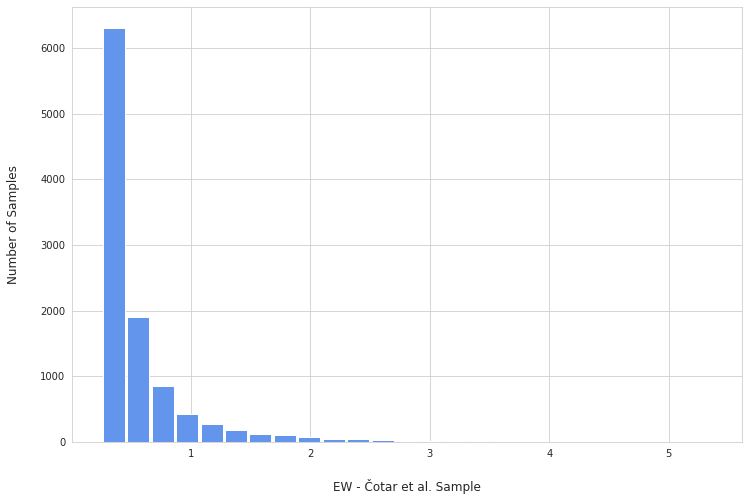
\includegraphics[scale=0.50]{figures/EW hist cotar.png}
\caption{The equivalent width (EW) distribution of the inverted difference spectra of the emission-line spectra provided by \citet{vcotar2021galah}. Here EW > 0.25. Note that this sample contains additional spectra not in GALAH DR3.}
\end{figure}

\begin{figure}[!htb]
\centering
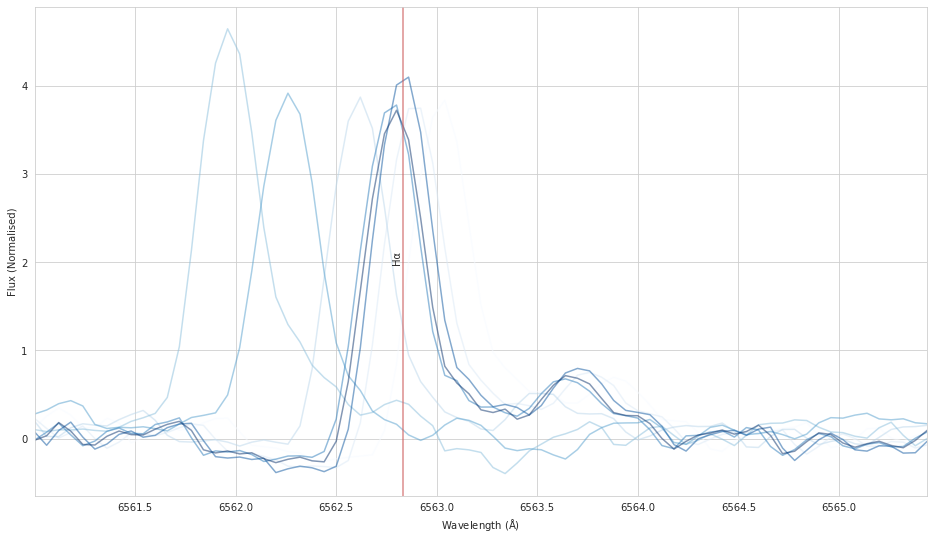
\includegraphics[scale=0.42]{figures/class_23_45.png}
\caption{Ensemble plot of 8 spectra with emission-lines superimposed on absorption}
\end{figure}

\begin{figure}[!htb]
\centering
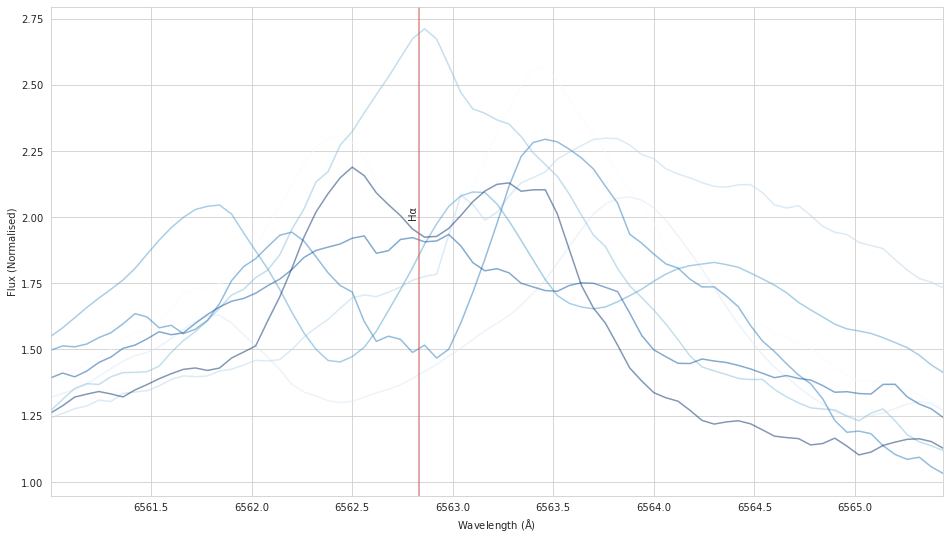
\includegraphics[scale=0.42]{figures/class_21_45.png}
\caption{Ensemble plot of 8 spectra with similar morphologies separated by DTW.}
\end{figure}

\begin{figure}[!htb]
\centering
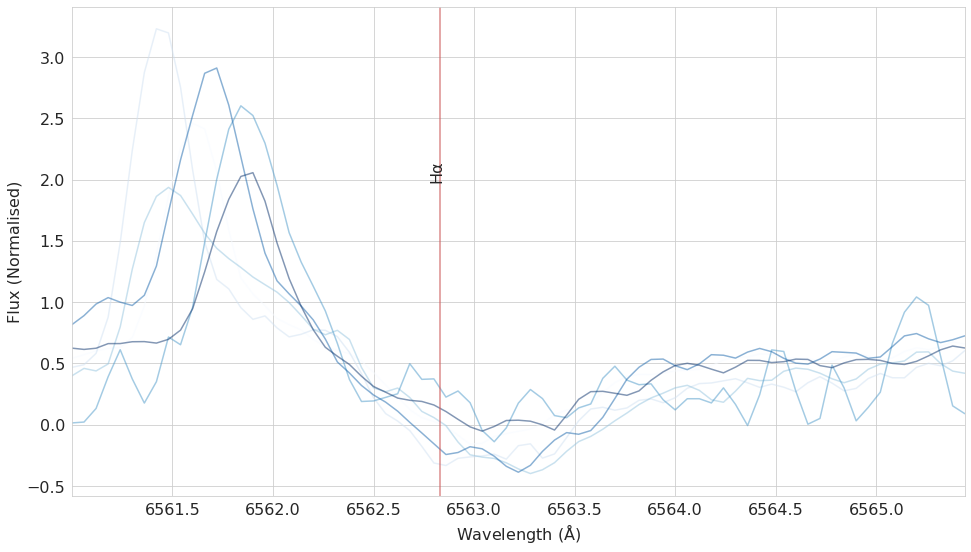
\includegraphics[scale=0.42]{figures/class_25_45.png}
\caption{Ensemble plot of 6 spectra with similar morphologies separated by DTW.}
\end{figure}

\begin{figure}[!htb]
\centering
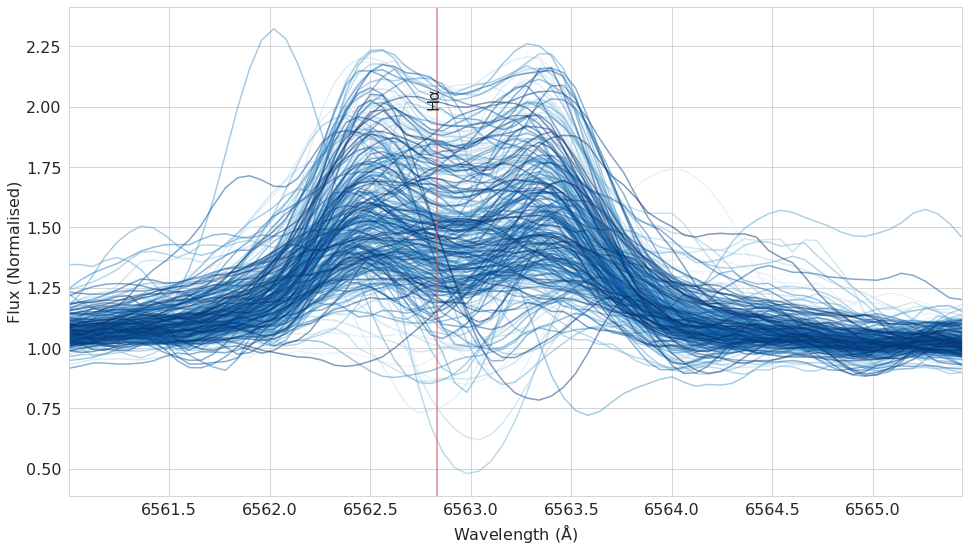
\includegraphics[scale=0.42]{figures/class_11_45.png}
\caption{Ensemble plot of 352 spectra with similar morphologies separated by DTW.}
\end{figure}




